%=========PROBLEM 2============================================
\section*{Mode: Add air resistance}

In this case, the golf ball in addition to the force of gravity will also feel a force that oppose its movement.
\begin{equation*}
    \Sigma F = F_gravity + F_air
\end{equation*}

This last force is the air resistance which will be simulated with a drag model such as the following:

\begin{equation}
    \Vec{F}_{air} = -C_d \frac{\rho A v^2 }{2}\frac{\Vec{v}}{|\Vec{v}|}
    \label{eq:drag}
\end{equation}

where $C_d$ is the drag coefficient, $\rho$ is the density of the air, $A$ is the surface area in contact with air, and $v$ is the velocity vector. Note that the air resistance is a force that opposes the movement. The differential equation that needs to be solve is,

\begin{equation*}
    \frac{dv}{dt}= \frac{\vec{F}}{m} - C_d \frac{\rho A v^2 }{2m}\frac{\Vec{v}}{|\Vec{v}|} = \vec{a}-Kv^2\frac{\Vec{v}}{|\Vec{v}|}
\end{equation*}{}
 where K is a constant $= \frac{C_d \rho A }{2m}$. 
 
To solve this equation, we use the same function of RK4 as before. Figure \ref{fig:airDiffAngleSamePos} shows 4 groups of three plots. 
Each of these plots show the behavior of different angles on the same conditions. They also include data to compare this mode, air drag, with the mode of gravity only. 
The top plot of each group is the trajectory in terms of x and y position. The first thing to note is that at first glance they follow different paths.
In other words, the air drag makes a big difference not just in the position but also in the time it takes to reach the final destination. 
The middle plot of each group shows the y position with respect to time. In this case, the y position of both models, gravity only and with air drag, are almost the same. 
This makes sense since the y component of the velocity is very small so it will make a small contribution toward the overall force sum. 
Contrary to the y position, the bottom plot of each group shows an x position very different. Again, this makes sense since our movement is mainly horizontal, the air resistance in this axis will have a big contribution against our movement. 
In addition to before, this plots show the time difference to which they reach their final destination. 
Finally, the aimed angle is more complicated to calculate but a simple trial and error of the angles show  that they are under \ang(1.5).  

\begin{figure}
    \centering
    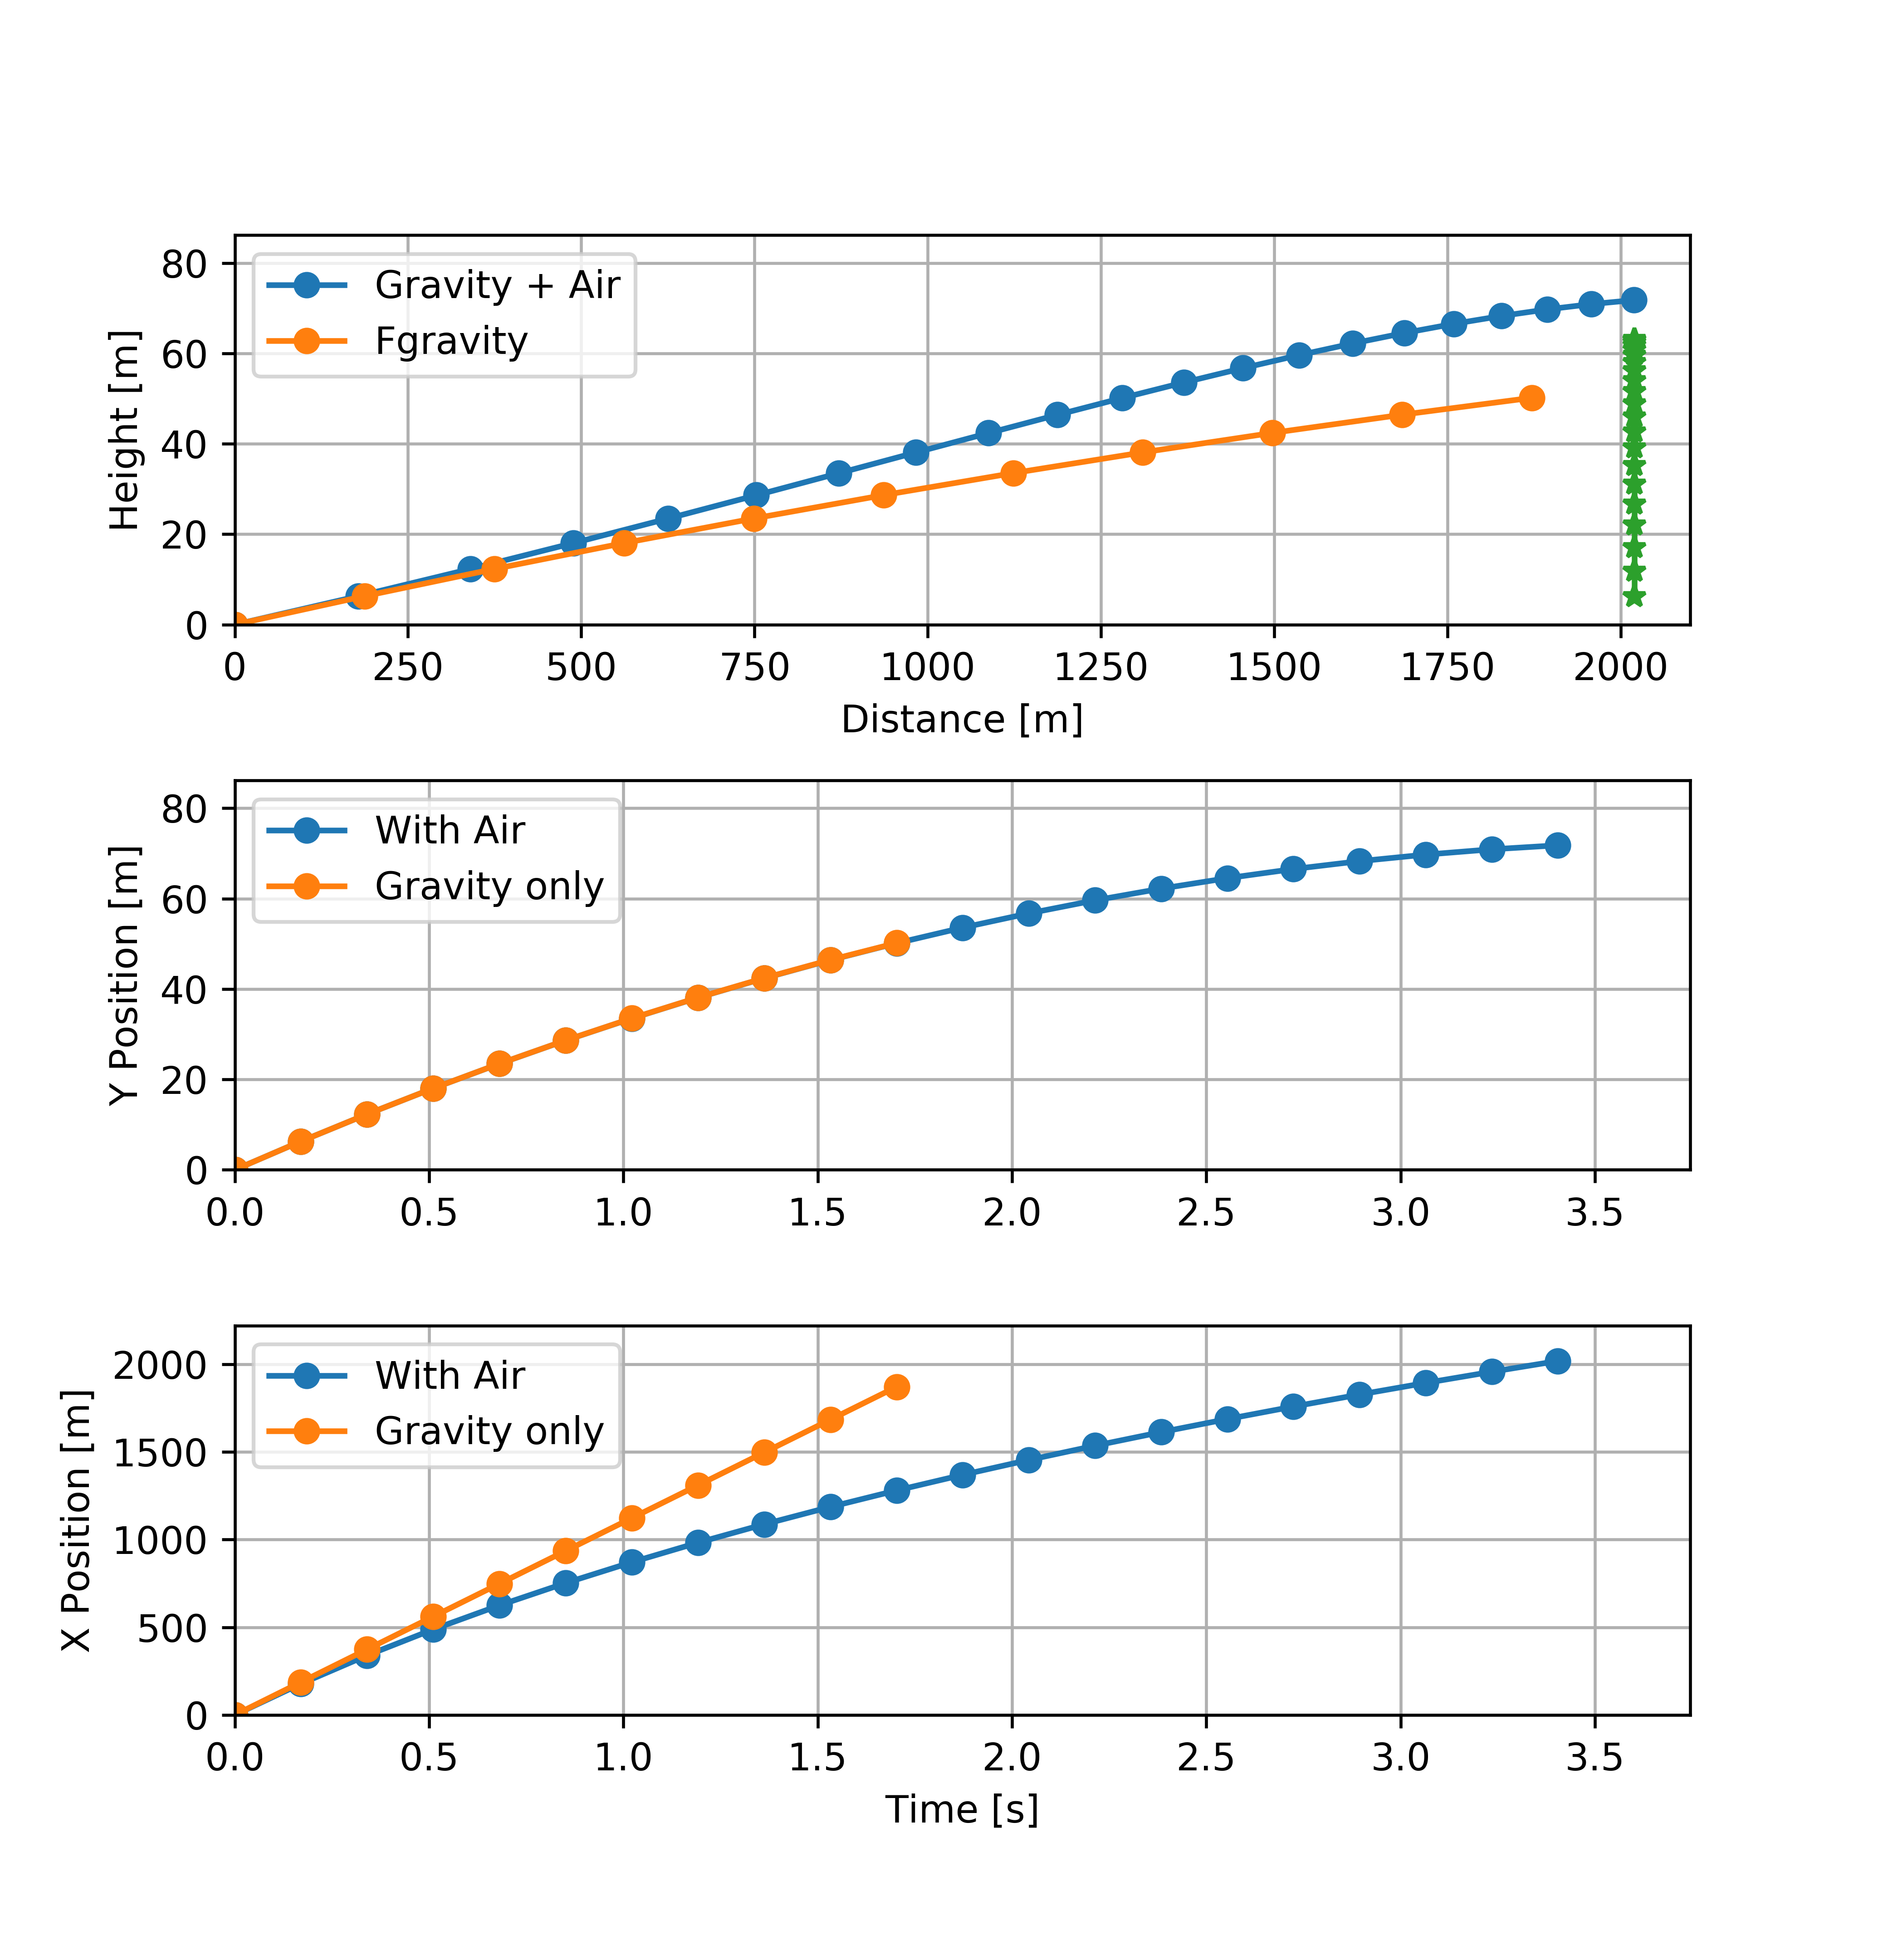
\includegraphics[width=.49\textwidth]{figures/aa1-97x2019-37y63-11.png}
    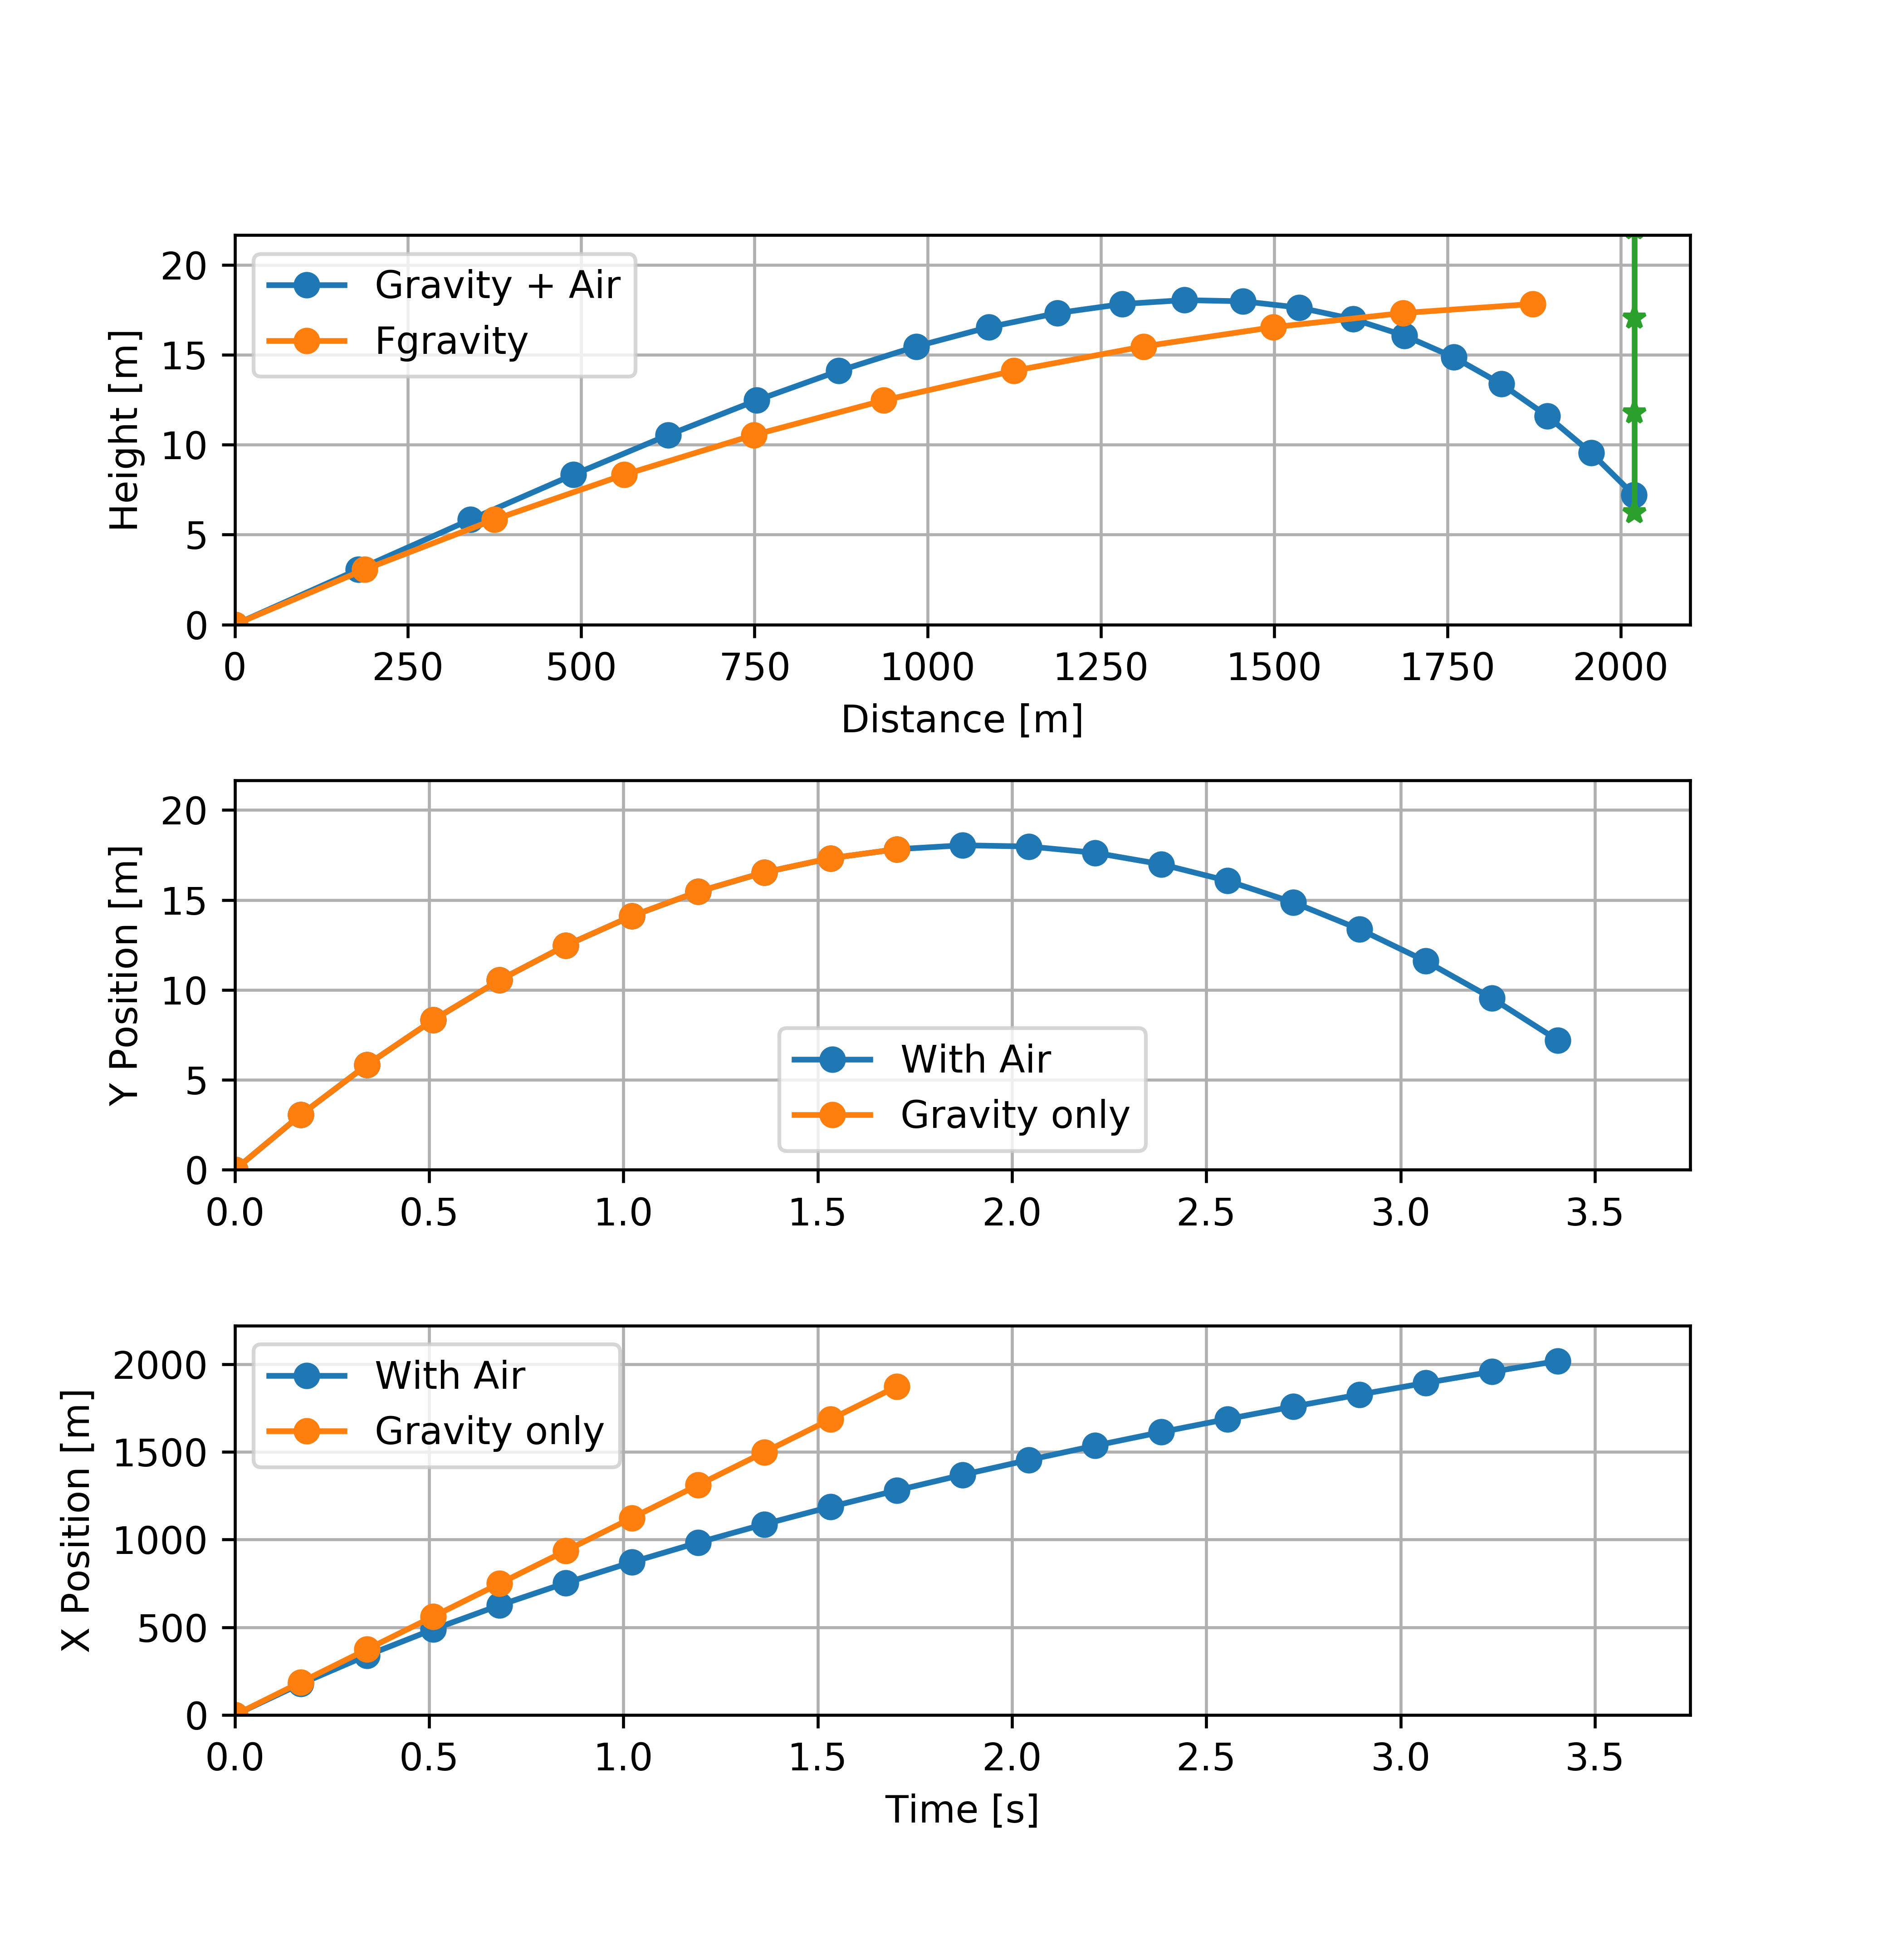
\includegraphics[width=.49\textwidth]{figures/aa0-98x2019-37y63-11.png}
    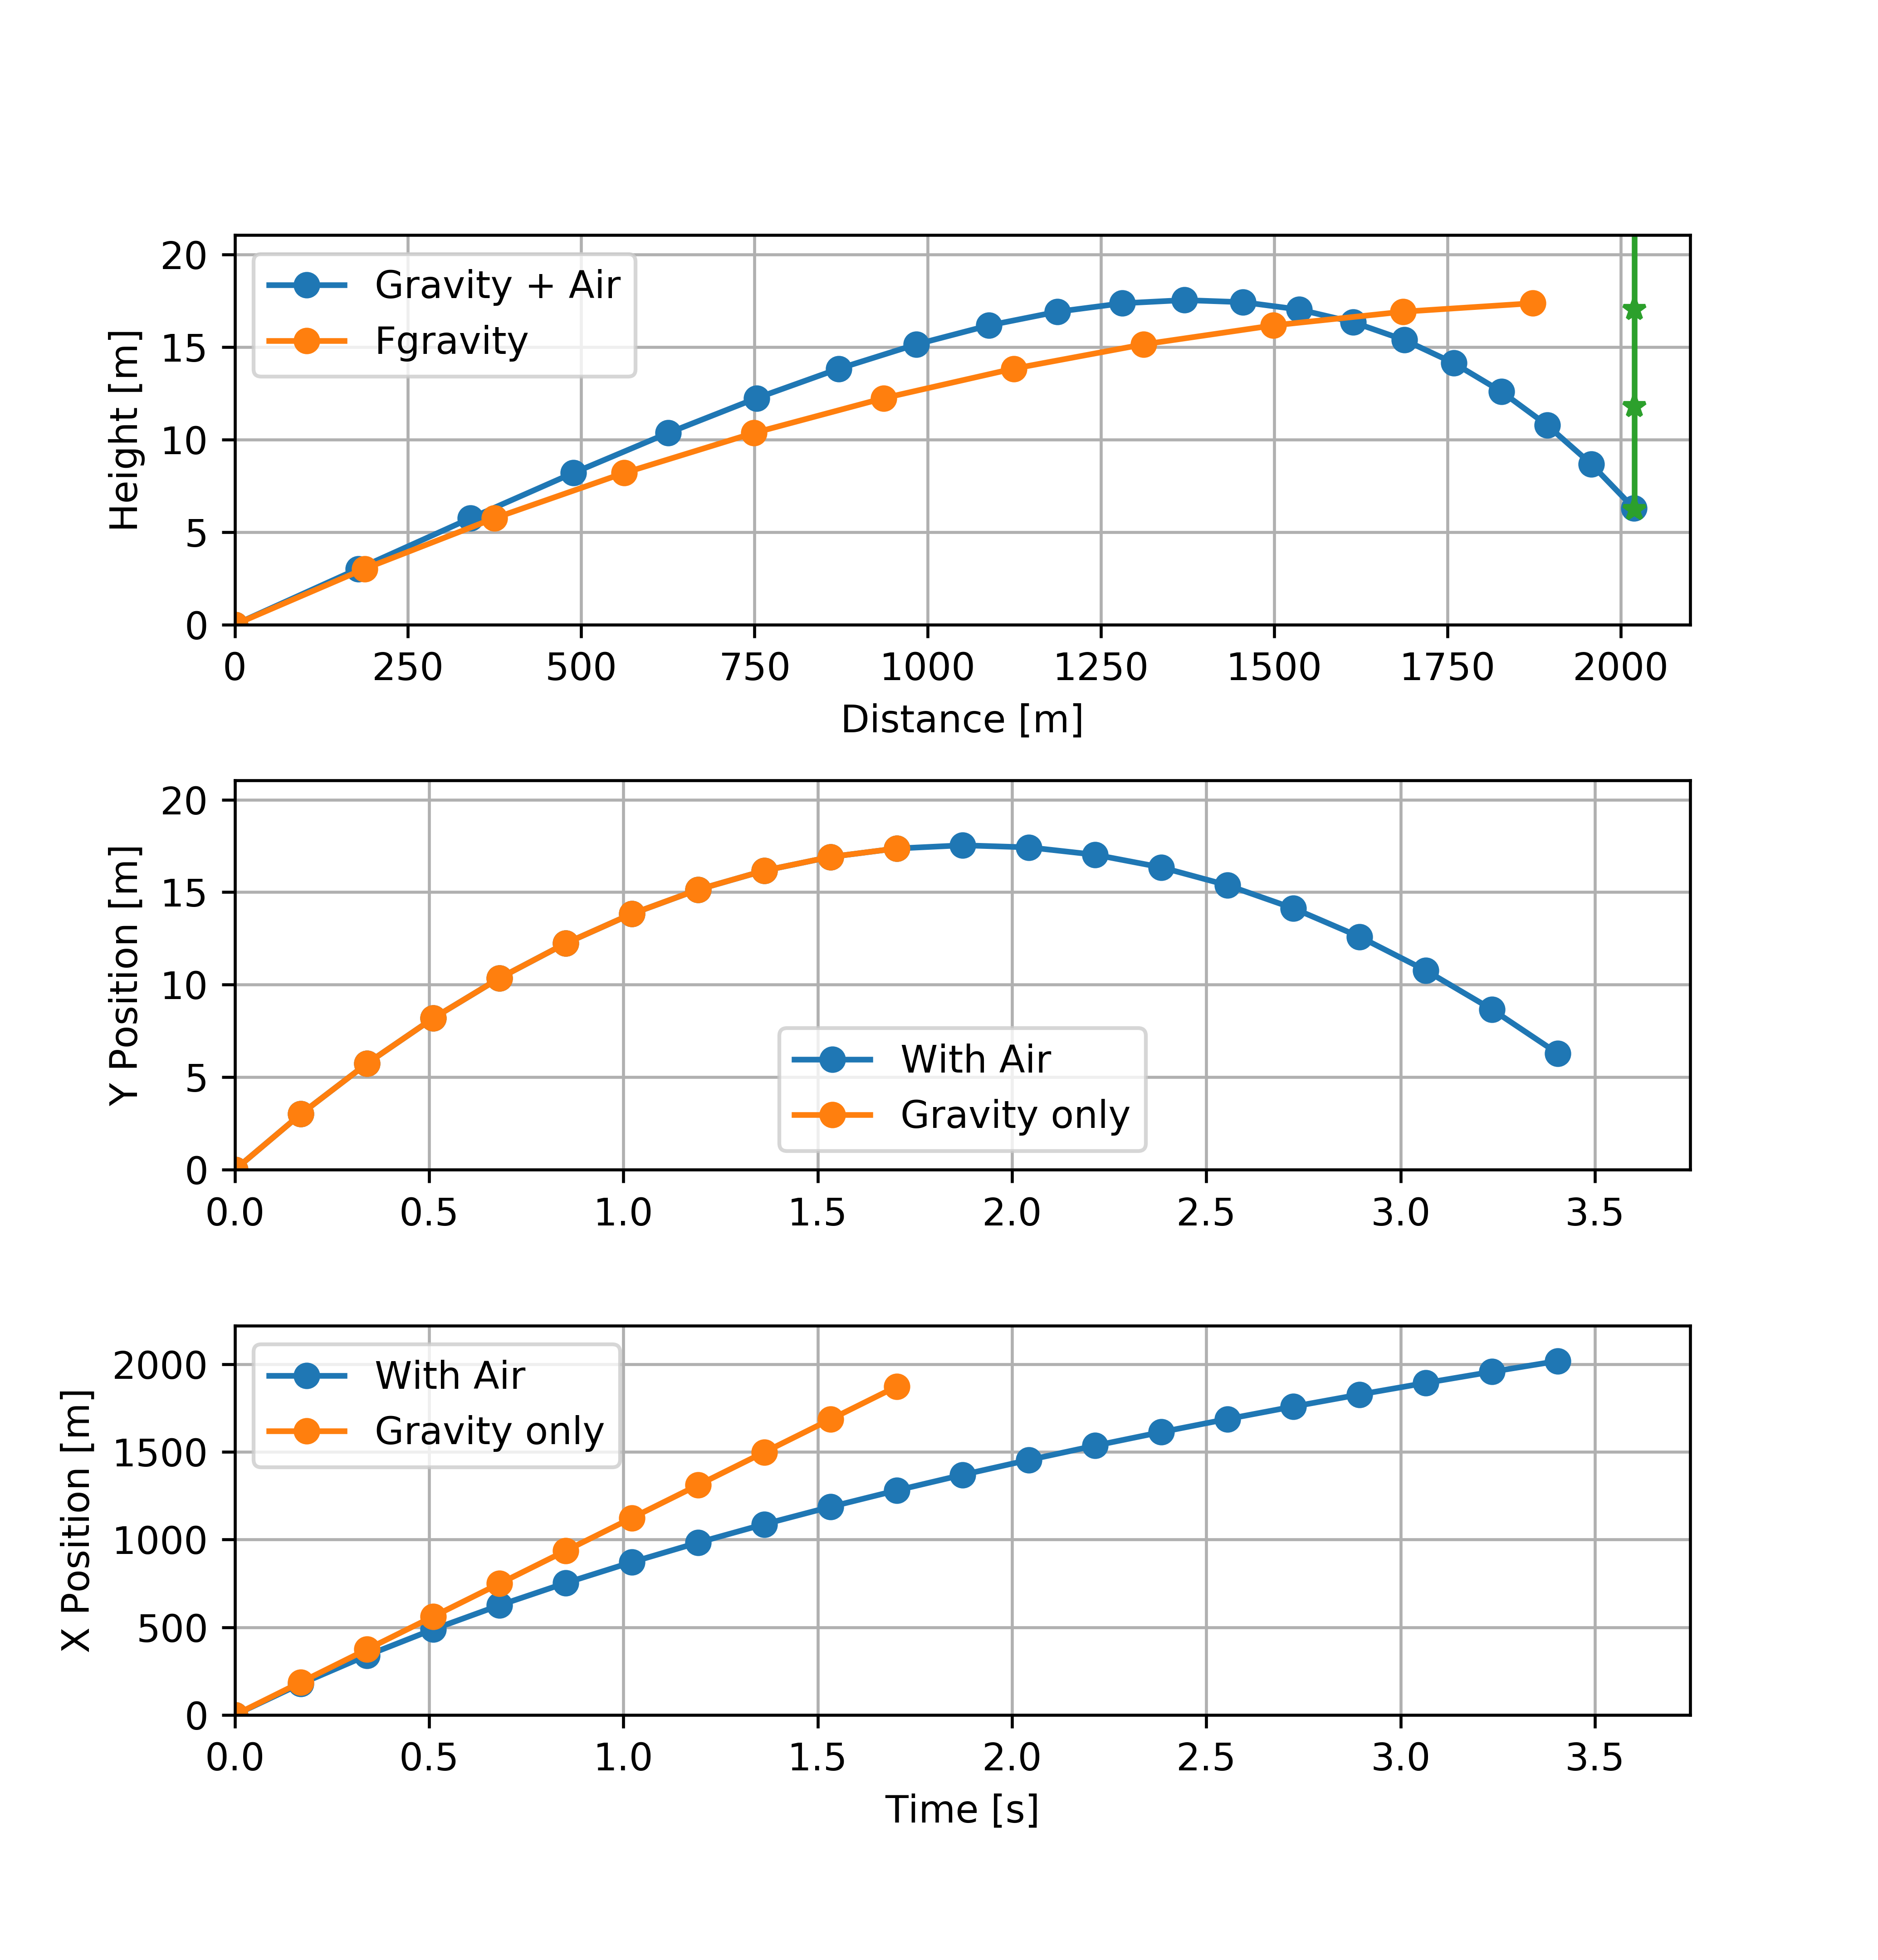
\includegraphics[width=.49\textwidth]{figures/aa0-966x2019-37y63-11.png}
    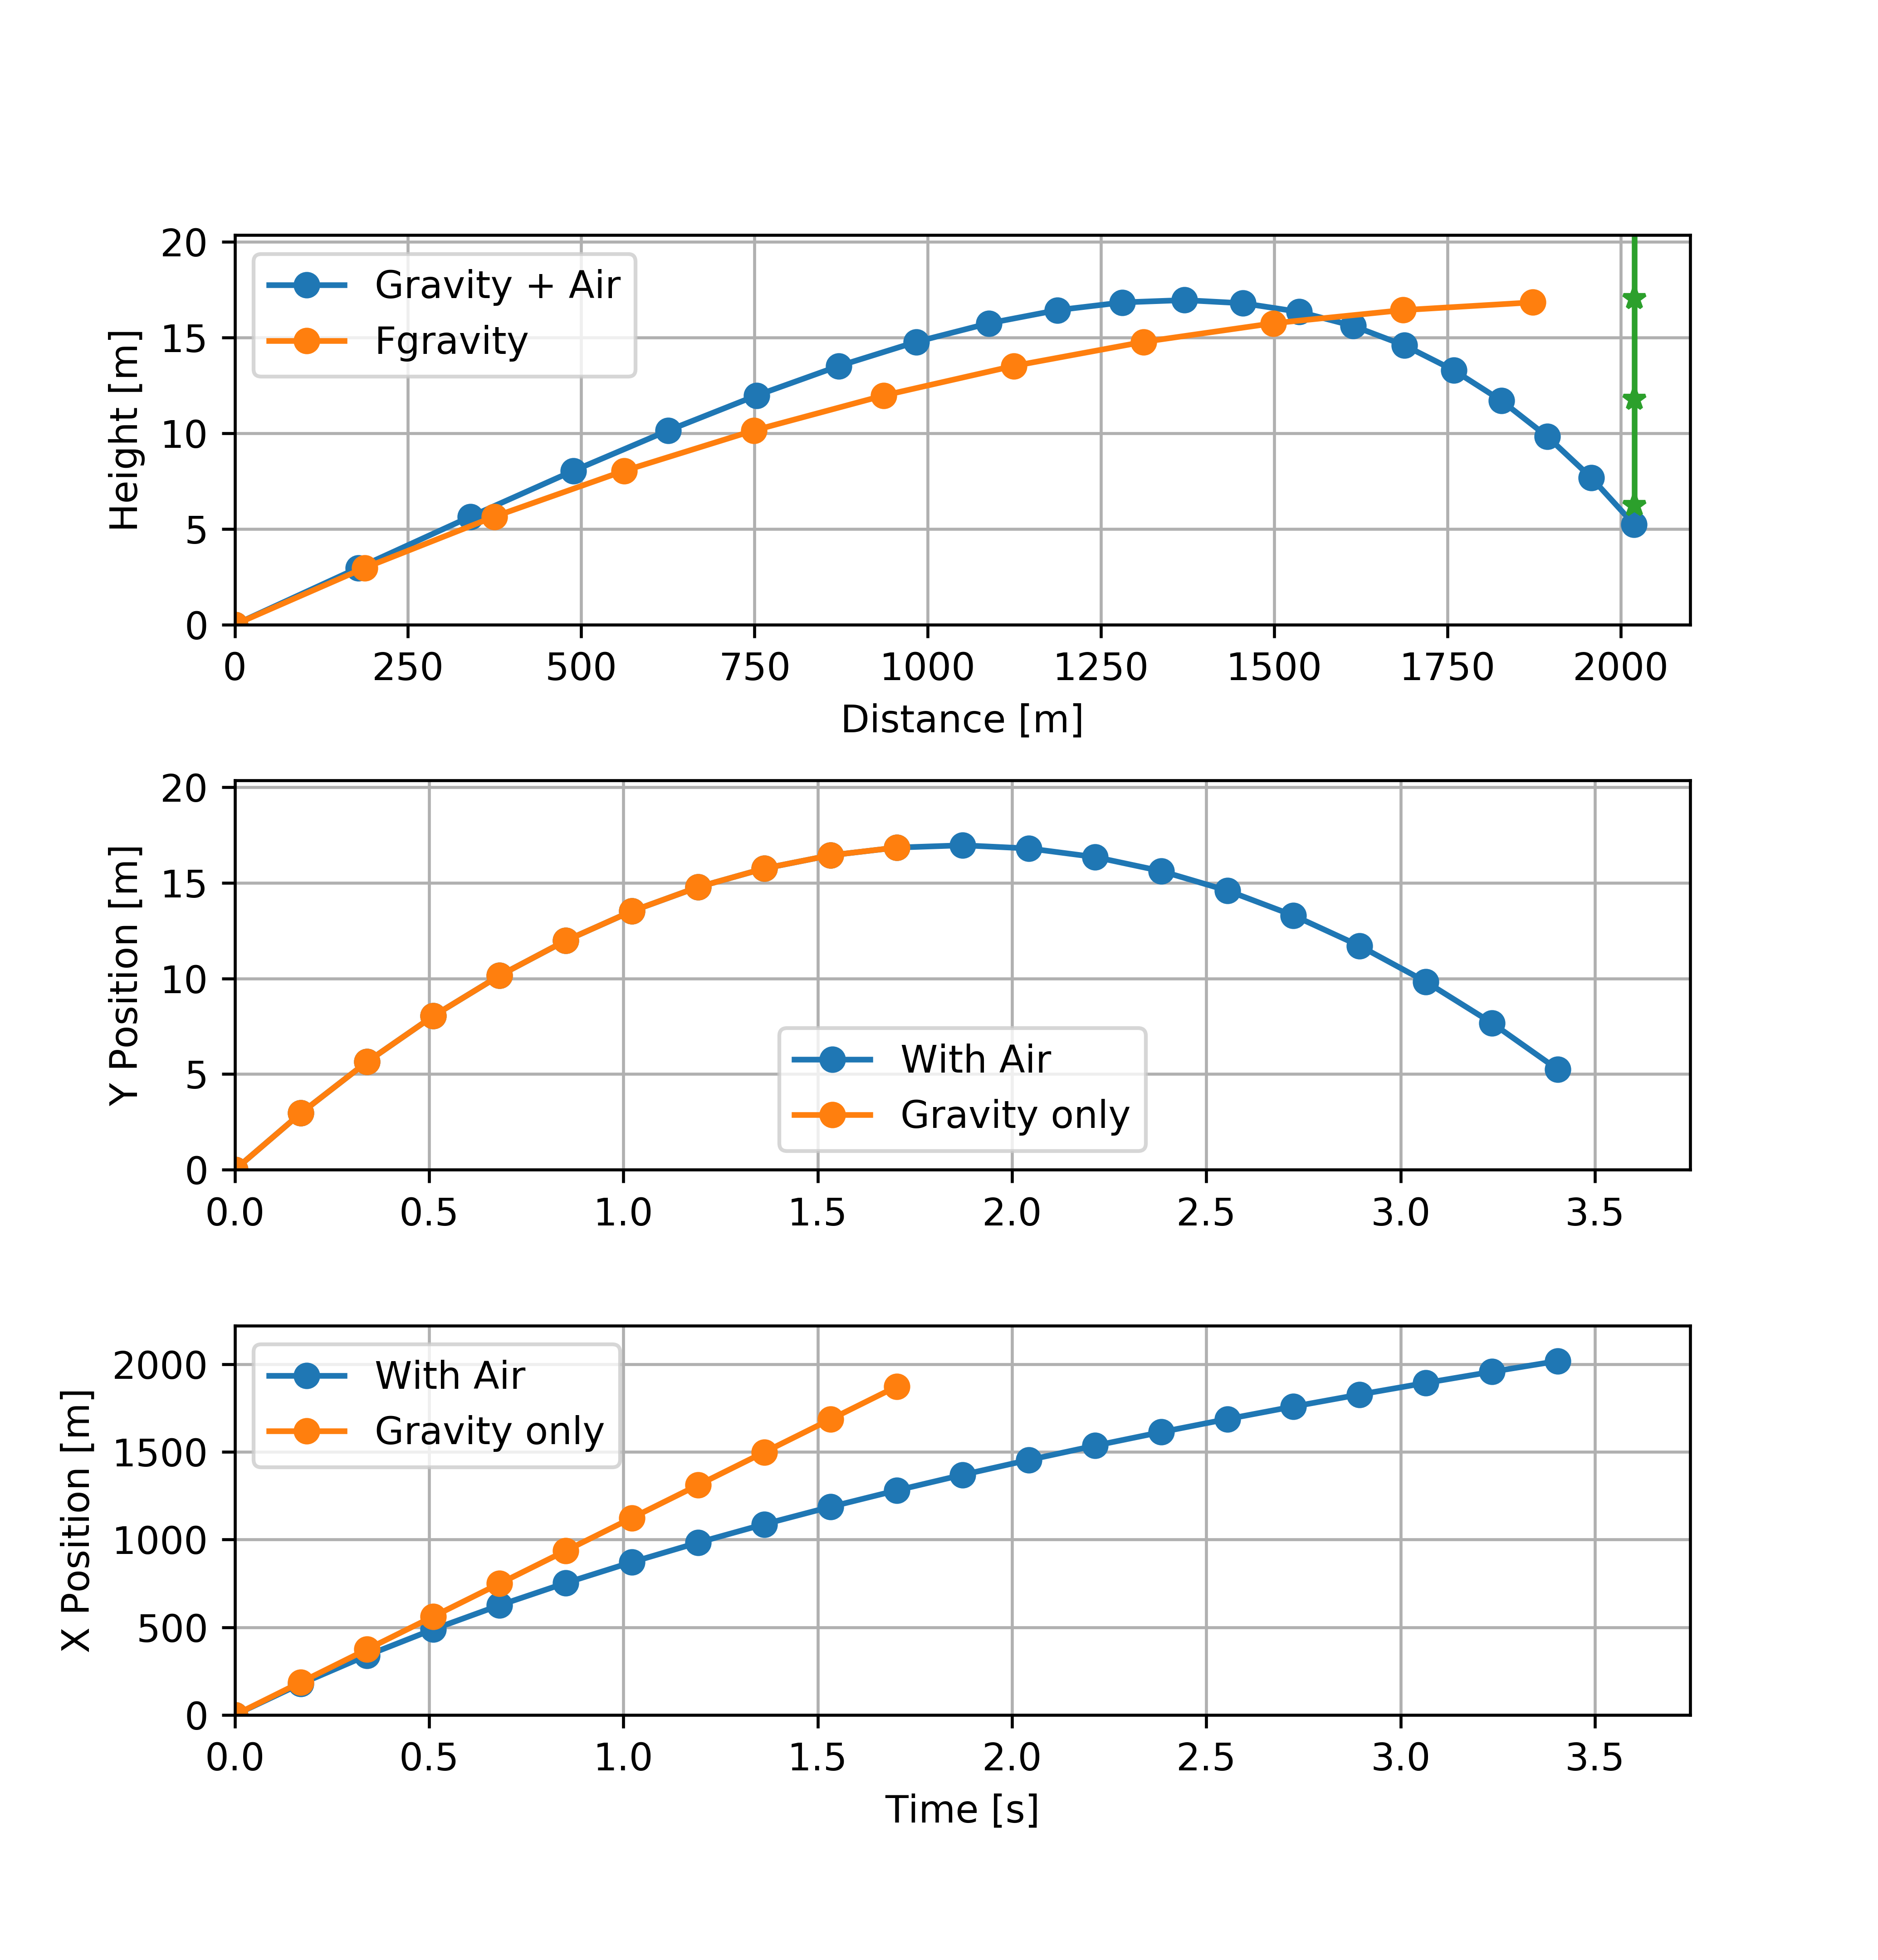
\includegraphics[width=.49\textwidth]{figures/aa0-95x2019-37y63-11.png}
    \caption{4 groups of three plots. Each plot corresponds to a different angle under the same conditions of distance from the monkey. Top Left: Angle \ang{1.970}. Top Right: Angle \ang{0.98}. Bottom Left: Angle \ang{0.966}. This was a HIT. Bottom Right: Angle \ang{0.95}.}
    \label{fig:airDiffAngleSamePos}
\end{figure}